\section{From Raw Products to Co-Registered Footprints}
\label{sec:dataset}

\begin{figure*}[t]
  \centering
  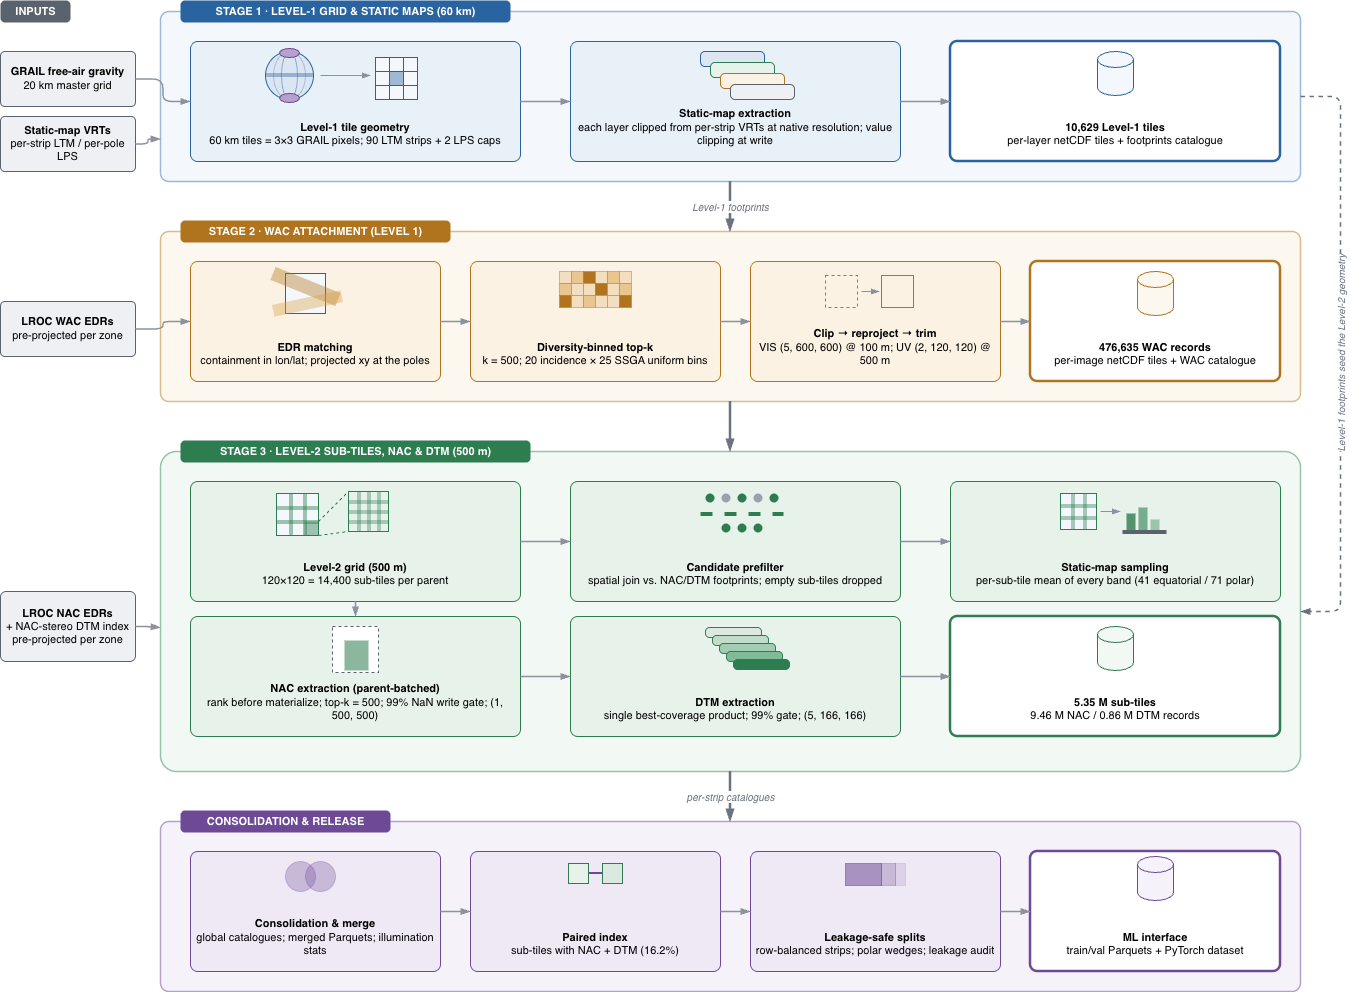
\includegraphics[width=\textwidth]{figures/footprint_anchored.png}
  \caption{Corpus construction. Stage~1 lays 60\,km footprints ($3\times3$ GRAIL pixels) over 90 LTM strips and two polar caps and clips every static layer at native resolution. Stage~2 keeps up to 500 illumination-diverse WAC observations per footprint. Stage~3 cuts each footprint into 500\,m sub-tiles that carry per-sub-tile static means, NAC images and the best stereo terrain model. Consolidation builds the merged and paired catalogs and the splits. Heavy borders mark stored artifacts.}
  \label{fig:pipeline}
\end{figure*}

SomBench~\cite{patil2026sombench} cuts its tiles inside individual image canvases, one view per tile, which suits benchmarks posed on one image. A world model needs the reverse: the ground is the sample and the images are views of it, aligned pixel for pixel under many suns. We reuse SomBench's raw image selection and preprocessing and build a different corpus on top (\cref{fig:pipeline,tab:contrast}). The supplement (\cref{sec:supp_data}) gives the long form of every stage and lists all 34 layers.

\begin{table}[t]
  \centering
  \footnotesize
  \setlength{\tabcolsep}{3pt}
  \caption{Two corpora built from the same raw products.}
  \label{tab:contrast}
  \begin{tabular}{@{}p{0.22\linewidth}p{0.36\linewidth}p{0.38\linewidth}@{}}
    \toprule
    & Image-anchored (SomBench) & Footprint-anchored (ours) \\
    \midrule
    Sample unit       & 512\,px window in one record      & 60\,km footprint, $3\times3$ GRAIL px \\
    Images per place  & one per tile                      & up to 500 on identical bounds \\
    Static layers     & re-clipped per record (42.5\,TB)  & once per footprint (9.5\,TB) \\
    NAC--WAC link     & independent tracks                & sub-tiles keyed to their parent \\
    Ground overlap    & windows may overlap               & none (seam ownership) \\
    Geometry          & one set per tile                  & per observation, plus series statistics \\
    \bottomrule
  \end{tabular}
\end{table}

\subsection{Source products and preprocessing}
\label{sec:sources}

Camera observations are experiment data records (EDRs) of the LRO Wide and Narrow Angle Cameras~\cite{robinson2010lunar}, drawn from the SomBench pools of 63,468 WAC and 11,302 NAC records, plus 585 NAC stereo terrain models (DTMs) at 2--5\,m~\cite{henriksen2017extracting}. Static layers come from ten instruments on four missions: SLDEM2015 topography~\cite{barker2016new}, LOLA roughness~\cite{kreslavsky2013lunar,neumann2015copernican}, WAC mosaics and TiO$_2$~\cite{speyerer2011lunar,boyd2012lunar,wagner2015new,sato2017lunar}, Kaguya MI reflectance, mineralogy and space weathering~\cite{ohtake2008performance,lemelin2016global,trang2019improved}, Diviner rock abundance, regolith temperature, H-parameter and bolometric temperature~\cite{paige2010lunar,powell2023high,hayne2017global,williams2017global}, Mini-RF radar~\cite{nozette2010lunar,fassett2024improved}, the USGS geologic map~\cite{fortezzo2020release} and GRAIL gravity~\cite{zuber2013gravity}. Fourteen more layers serve the polar caps~\cite{williams2019seasonal,schorghofer2020mapping,mazarico2011illumination,lemelin2016improved,lemelin2022compositional,lawrence2022global}.

\paragraph{Preprocessing.}
\label{sec:preprocessing}
As in SomBench, EDRs are calibrated~\cite{mahanti2016inflight,humm2016flight} and echo-corrected with USGS ISIS\footnote{\url{https://doi.org/10.5066/P13YBMZA}} and orthorectified onto SLDEM2015 with the Ames Stereo Pipeline~\cite{beyer2018ames}. Each image is projected into the Lunar Transverse Mercator (LTM) zone~\cite{mcclernan2025lunar} holding most of its area. Static maps are harmonized to equidistant cylindrical and exposed as one virtual raster (VRT) per LTM strip and per Lunar Polar Stereographic (LPS) cap.

\subsection{Footprints on the GRAIL grid}
\label{sec:grid}

GRAIL gravity at 20\,km is global and independent of illumination, so it is the master grid. A Level-1 footprint is a $3\times3$ block of GRAIL pixels, 60\,km on a side in its region's projection and aligned to GRAIL pixel edges, so the master grid is never resampled. The regions are 90 LTM strips of $8^\circ$ longitude, 45 per hemisphere up to $|\phi|{=}82^\circ$, and two LPS caps; zones 1 and 45 are inset $0.5^\circ$ from the antimeridian. Footprints are laid without overlap, which would only duplicate: static pixels on shared ground are identical, and a WAC record clipped twice keeps its geometry.

\paragraph{Seam ownership.} A footprint belongs to the region holding its center. Each region tiles its own projected raster, so edge footprints of neighboring regions could cover up to 94\% of the same ground. Of two overlapping candidates from different regions we create only the one with more of its area inside its own region, with ties to a fixed region ranking. Each strip job derives its neighbors' candidates from their GRAIL rasters, so the 92 jobs stay independent. Over the $0$--$82^\circ$ band, the center rule covers 94\% of the ground with 5.9\% twice; ownership covers 82\% with none twice. \TODO{refresh counts after the seam repair; \cref{tab:corpus} predates it}

\subsection{Static layers once per footprint}
\label{sec:attach}

A layer of native resolution $r$ is read from the strip's VRT, already in the footprint's projection, and clipped at native pixels to a side of $t = \lfloor 60\,\text{km}/r \rfloor$, from 1000 for SLDEM2015 to 3 for GRAIL. Nothing is reprojected; only GRAIL and Diviner bolometric temperature are resampled within the same projection to restore the $t\times t$ shape. Each layer is extracted once per footprint and shared by all its observations and sub-tiles. SomBench re-clips every layer for every image tile and stores 21.5\,M files in 42.5\,TB; this corpus takes 9.5\,TB.

At write time, categorical bands are snapped to their classes, circular bands wrapped, and every band clipped to its physical range, with NaN kept as a gap. A scan of all sources showed that cubic resampling in the VRTs smeared no-data sentinels into neighbors (FeO up to 2,810\,wt\%, aspect up to $450^\circ$), and found eleven defective NAC products, which are excluded (\cref{sec:supp_data}).

\subsection{Repeat observations with their geometry}
\label{sec:wac}

\begin{figure}[t]
  \centering
  \begin{subfigure}[t]{0.49\linewidth}
    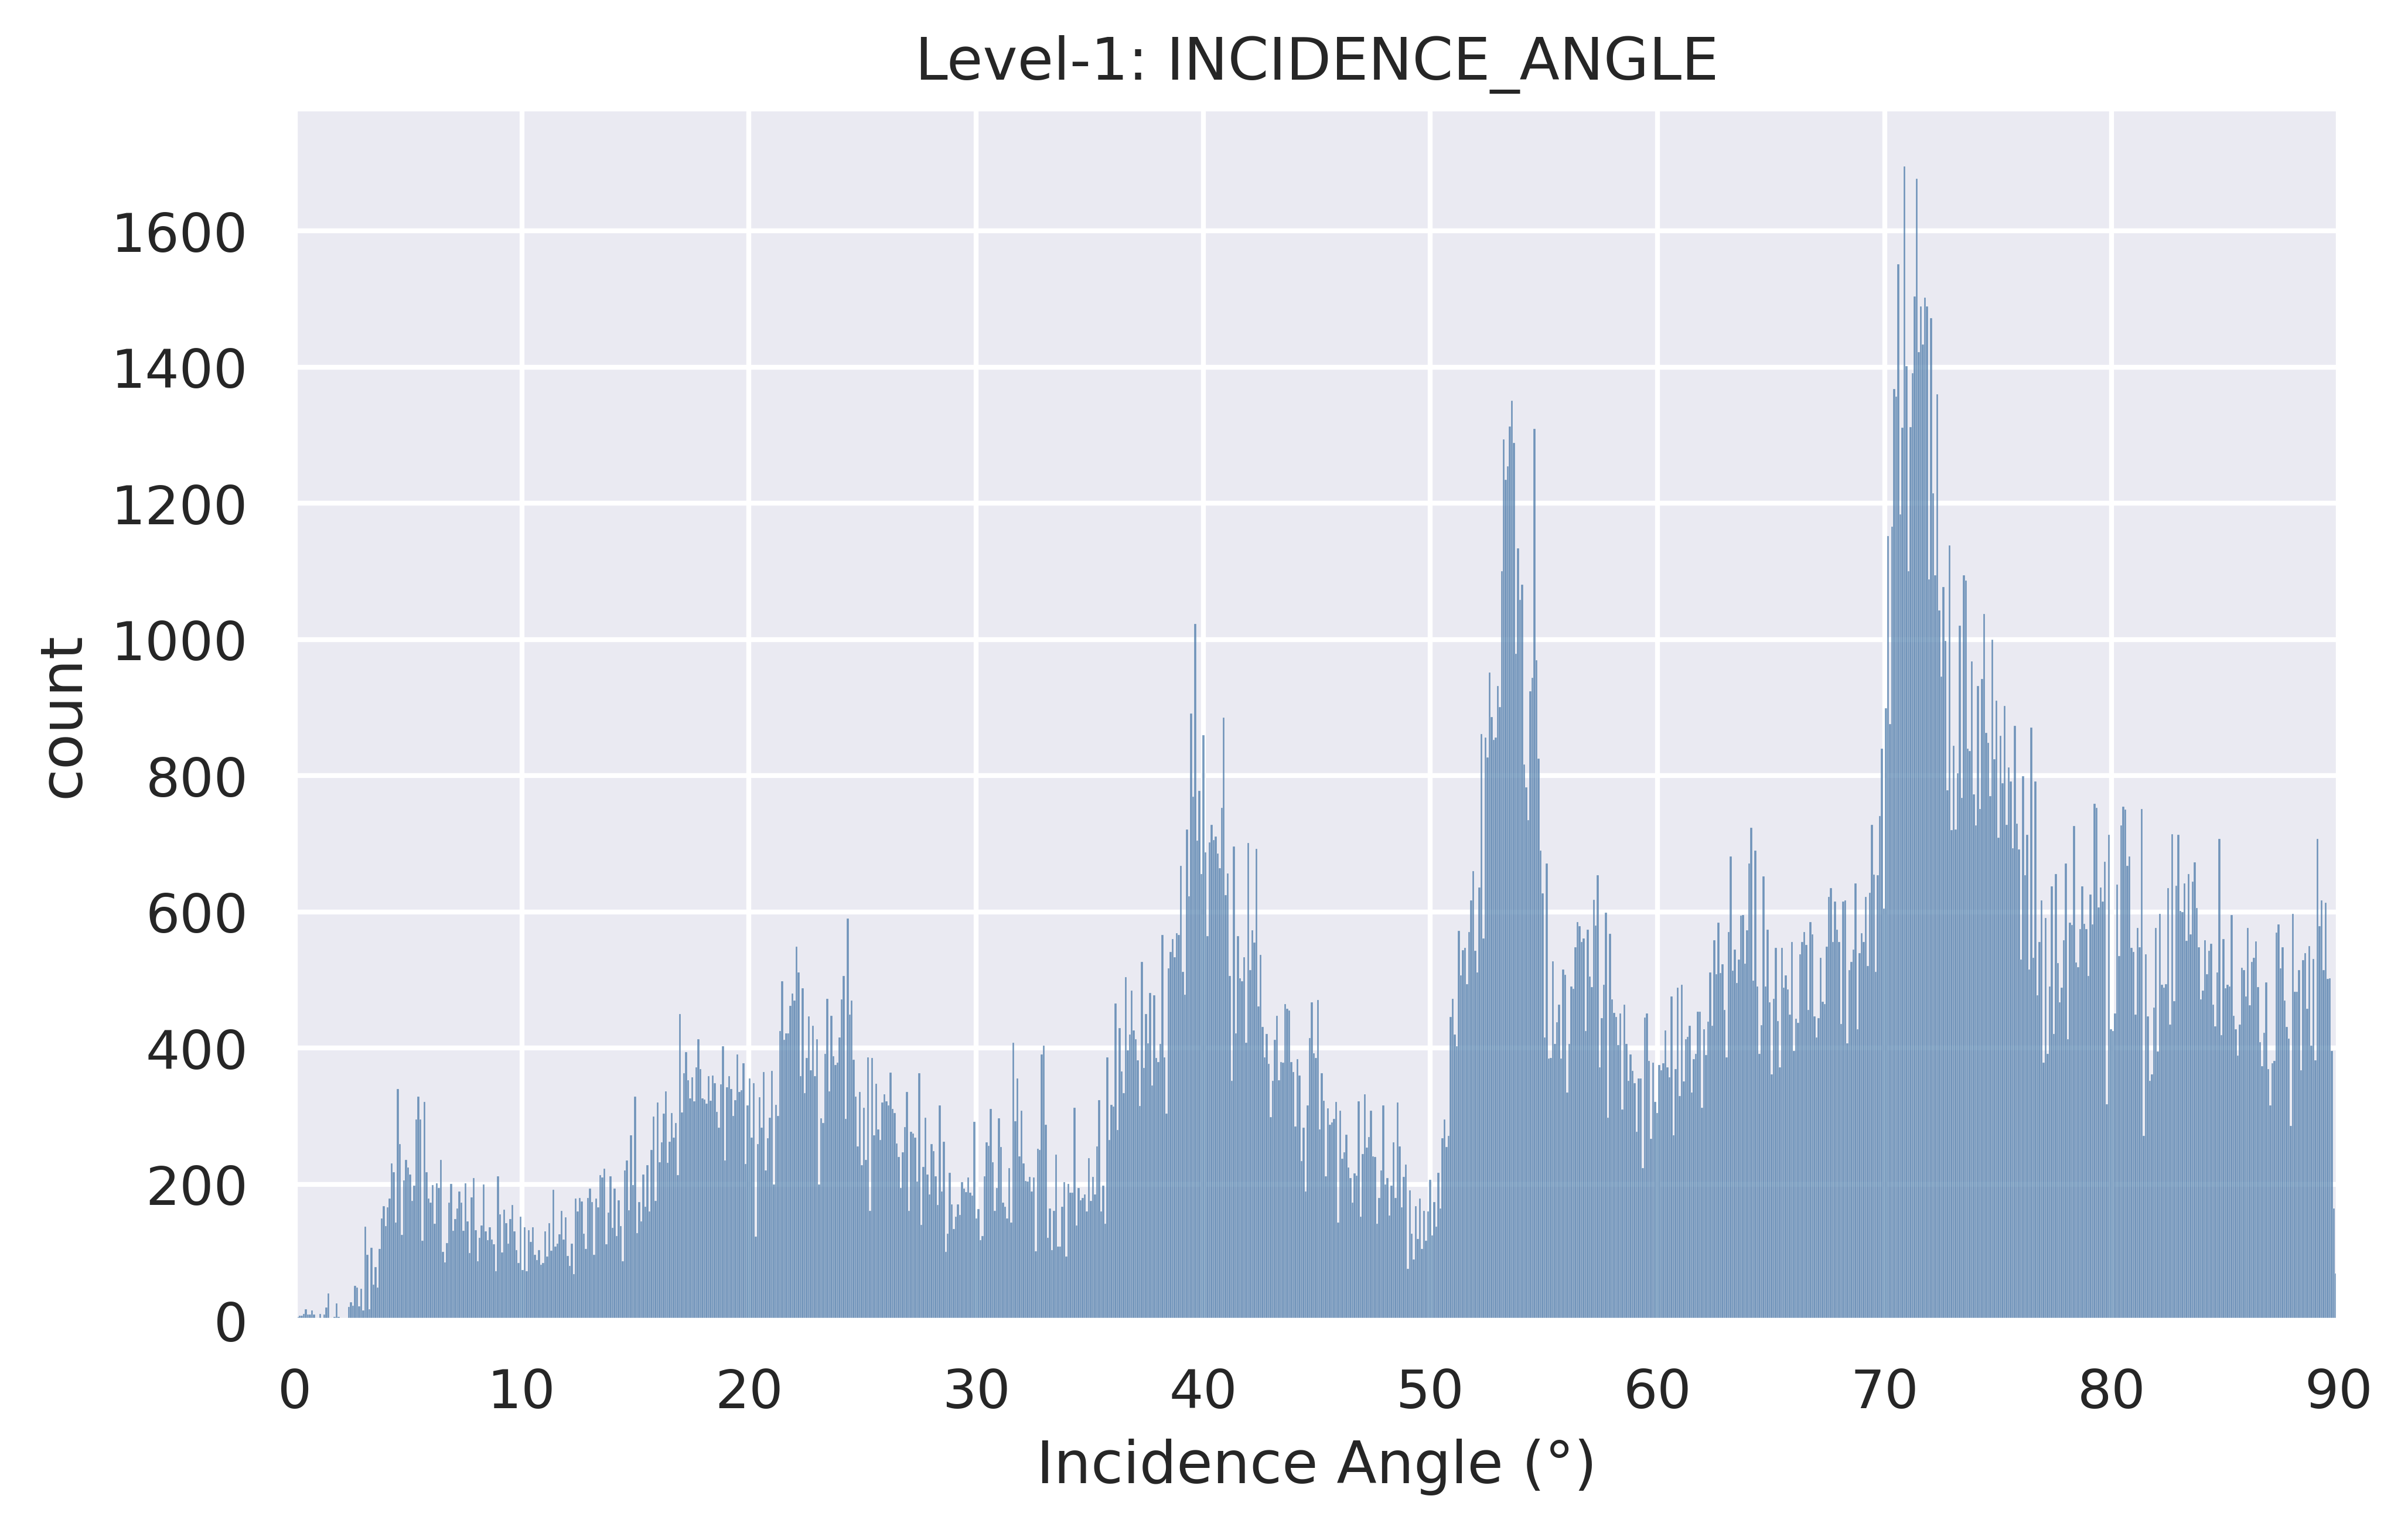
\includegraphics[width=\linewidth]{figures/level1_INCIDENCE_ANGLE.png}
    \caption{Incidence angle.}
  \end{subfigure}\hfill
  \begin{subfigure}[t]{0.49\linewidth}
    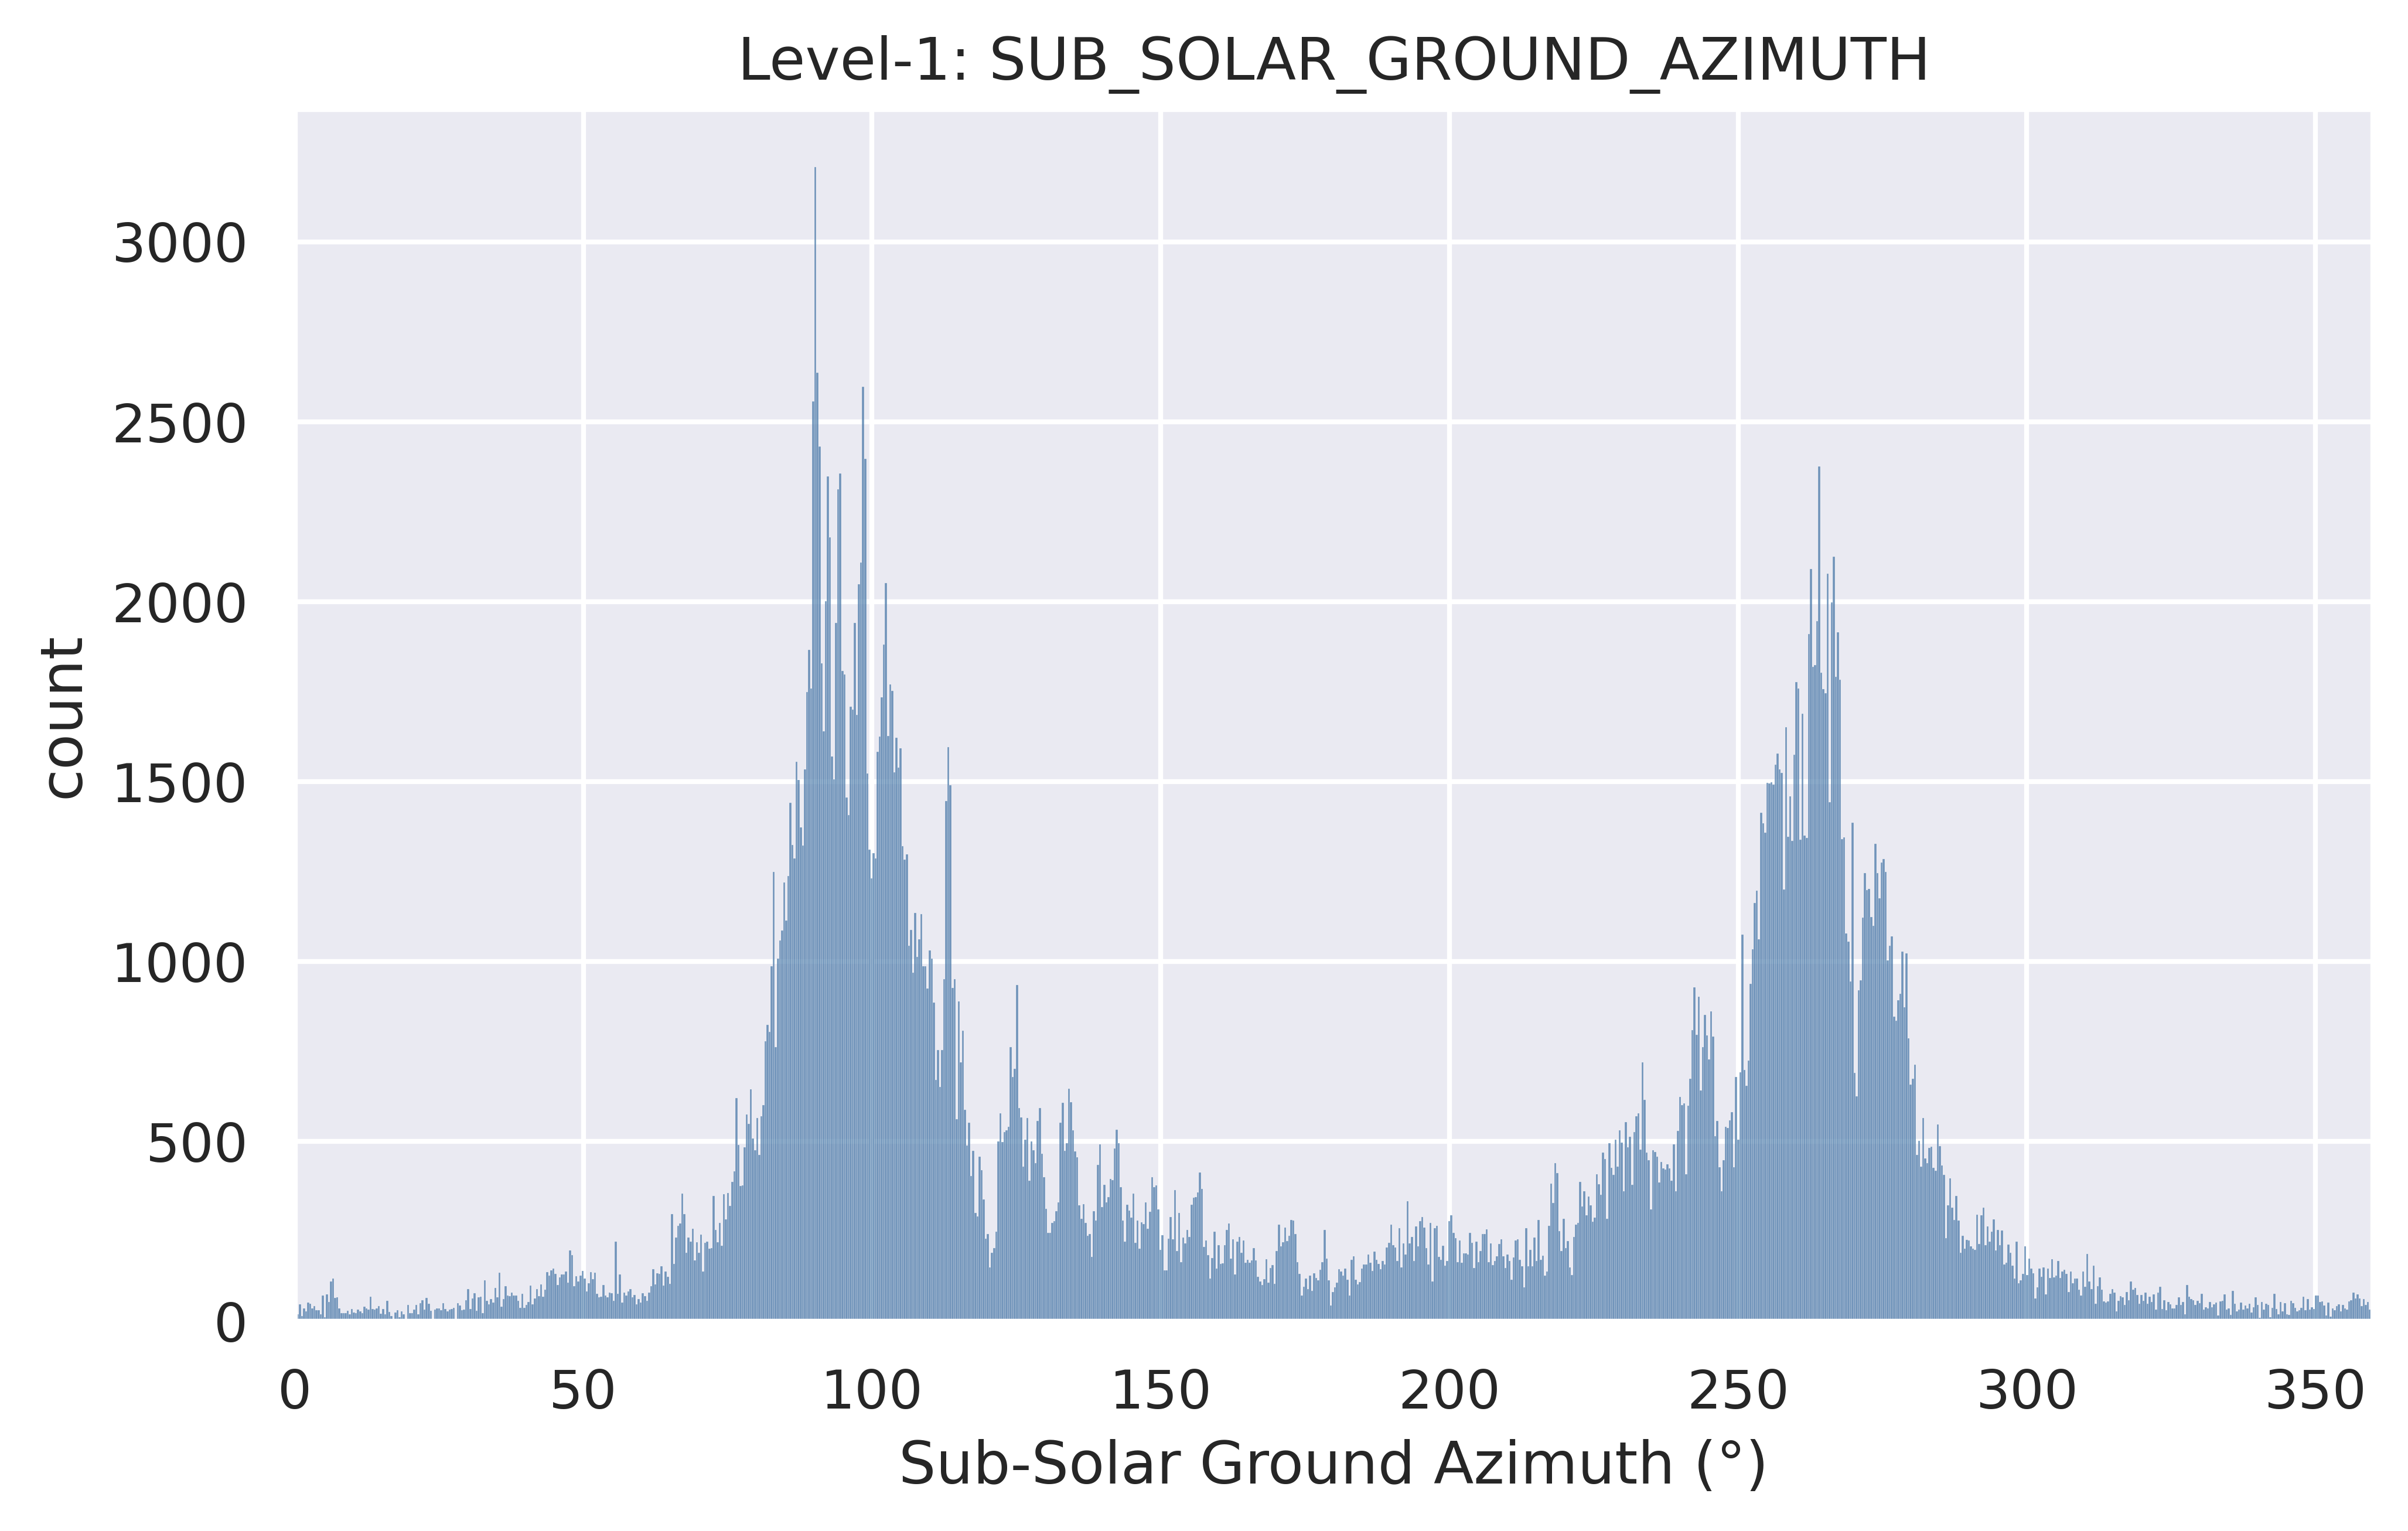
\includegraphics[width=\linewidth]{figures/level1_SUB_SOLAR_GROUND_AZIMUTH.png}
    \caption{Sub-solar ground azimuth.}
  \end{subfigure}
  \caption{Illumination of the 476,635 retained WAC observations. Incidence covers nearly the full $0$--$90^\circ$ range. Azimuth has two modes near $90^\circ$ and $265^\circ$, with smaller counts elsewhere.}
  \label{fig:illum}
\end{figure}

A WAC record is a candidate when its footprint polygon contains the footprint, tested in geographic coordinates, or in LPS coordinates in the caps, where a 60\,km square unprojects to a box hundreds of degrees wide. A record in the footprint's zone is sliced directly. Otherwise the four tile corners are transformed into the record's projection and enveloped, the record is clipped there with a 2-pixel buffer, and only the clip is reprojected and trimmed; incompatible pairs, such as a polar stereographic record and an LTM tile, are rejected.

Up to $k{=}500$ candidates are kept per footprint. They are binned by incidence (20 bins) and sub-solar azimuth ($\operatorname{round}(k/20){=}25$ bins), with edges from each strip's observed range, and drawn round-robin across occupied cells in random order, with five attempts per slot. A record with any missing visible or ultraviolet pixel is rejected. The final pass takes the lowest-NaN candidate of each cell first, so the set spans the sun instead of collapsing onto the cleanest, often near-duplicate, records. An observation is a visible $(5, 600, 600)$ tile at 100\,m and an ultraviolet $(2, 120, 120)$ tile at 500\,m, with incidence, emission, phase, sub-solar azimuth, sub-solar and sub-spacecraft coordinates and north azimuth. The corpus holds 476,635 WAC observations; 86.9\% of footprints have at least one, and a covered footprint has about 52 (\cref{fig:illum}).

\subsection{Sub-tiles with NAC and stereo terrain}
\label{sec:level2}

On a 60\,km footprint, NAC at 1\,m would need 60,000 pixels per side and a swath covers only part of it. Each parent is therefore cut into $120\times120$ sub-tiles of 500\,m with a parent key. A spatial join drops sub-tiles with no NAC or DTM candidate before any raster is read, and an averaging read of the parent gives every static band as a per-sub-tile mean (41 bands equatorial, 71 polar).

NAC observations are chosen by the same sampler and placed at their true position in a $(1, 500, 500)$ canvas, so partial coverage stays NaN; canvases above 99\% NaN are not written. Each product is opened once per parent, and a first pass counts valid pixels per sub-tile without building canvases. Only the selected pairs are then materialized, avoiding about $5\times10^8$ naive clip-and-reproject operations. Each sub-tile also gets the DTM with the lowest elevation NaN: elevation, slope, aspect and its sine and cosine at $(5, 166, 166)$. Of the 5,354,773 retained sub-tiles, 86.6\% have NAC and 16.0\% a DTM.

\subsection{Records and splits}
\label{sec:splits}

\begin{table}[t]
  \centering
  \footnotesize
  \setlength{\tabcolsep}{4pt}
  \caption{Configuration and scale. Coverage is the share of footprints (WAC) or sub-tiles (NAC, DTM) with at least one record. Counts predate the seam repair of \cref{sec:grid}; the paired count also predates the NAC exclusion.}
  \label{tab:corpus}
  \begin{tabular}{@{}lr@{}}
    \toprule
    Regions                    & 90 LTM strips + 2 LPS caps \\
    Master grid                & GRAIL, 20\,km \\
    Footprint (Level 1)        & 60\,km, $3\times3$ GRAIL px \\
    Sub-tile (Level 2)         & 500\,m, $120\times120$ per parent \\
    WAC per footprint          & $k{=}500$, diversity-binned \\
    NAC per sub-tile           & $k{=}500$, diversity-binned \\
    DTM per sub-tile           & 1, lowest elevation NaN \\
    NaN gate                   & WAC 0\%; NAC, DTM 99\% \\
    \midrule
    Footprints                 & 10,629 \\
    Sub-tiles with NAC or DTM  & 5,354,773 \\
    WAC observations           & 476,635 (86.9\%, $\approx$52 each) \\
    NAC observations           & 9,453,706 (86.6\%) \\
    DTM tiles                  & 856,535 (16.0\%) \\
    Paired NAC + DTM rows      & 1,653,060 \\
    Source WAC / NAC products  & 59,503 / 10,484 \\
    Compressed size            & 9.5\,TB \\
    \bottomrule
  \end{tabular}
\end{table}

Per-strip Parquet catalogs are unioned into a Level-1 index (one row per footprint and WAC observation), a Level-2 index (one row per sub-tile and NAC observation, with the sub-tile's observation count and incidence and azimuth ranges) and a paired NAC and DTM index. Each layer of each tile is a compressed netCDF file with named bands, coordinates and projection.

Splits assign whole LTM strips to train, validation or test, accumulated greedily by row count so that dense strips do not skew the fractions; sub-tiles inherit their parent's split. Each cap is cut into eight longitude wedges, with parents beyond $88^\circ$ pinned to train. The splitter audits records that straddle a strip boundary and refuses splits whose footprints share ground. Pretraining in this paper uses the non-polar Level-1 rows (\cref{tab:corpus}). \TODO{non-polar train and validation footprint counts}
